\chapter{WebAssembly {\&} WebAssembly System Interface}
This chapter gives insight in what \acrfull{Wasm} is and how it works, alongside additional insight in how the \acrfull{WASI} works and how it is progressing.

\section{\acrshort{Wasm}}

When the web was born, the only supported programming language supported on the web was Javascript. As a relatively simple and portable language this did suffice. Over the years the web has become more complex and has become the center of the personal computer. However, its supported technologies did not grow at the same expansion pace. Javascript is still the only supported language and hampers the further expansion of the web. New technologies have been created to fix this issue, but none have succeeded. 
In order to be a viable Javascript alternative, a new model needs to be safe, fast, portable and compact. \acrshort{Wasm} is the first new technology to check all these four boxes. \cite{bringing_the_web_up_to_speed}

\subsection{Safe}
Wasm is intended to run in various environments, with some executing Wasm code from unknown sources. The web is a prime example of such a case. In these cases, it is required that the code runs in a sandbox, so that it cannot access all resources of the device. This way, malicious code can only do harm in the sandbox, and not the entire device.

Additionally, a Wasm program is often build in multiple modules. A Wasm module can be seen as an island of code, which imports and exports functions. Each module has its own stack, memory, types and more. This means that each module is isolated and cannot affect other modules, increasing the security of the model. Additionally, Wasm makes use of a linear memory model (Figure \ref{fig:wasm_high_level}). Each module gets its own range, and can only access that part of the memory.

\subsection{Portable}
\acrfull{Wasm} works as a compilation target for programming languages. Languages can compile to Wasm, just like they would for e.g. x86.
To compile to Wasm, the source code is first compiled to an intermediate representation, such as the LLVM IR. This is universal and also happens when compiling to other architectures. This part of the compilation process, called the frontend, stays the same. The backend of the compilation process, where the code gets translated into machine instructions, differs per instruction set. In the backend of the compiler the code will get compiled to the Wasm instruction set and output Wasm bytecode. This binary can get executed by a Wasm runtime. (Figure \ref{fig:wasm_compiler_frontend}) The bytecode is platform-agnostic, so it can run on any hardware and operating system that has a Wasm runtime. This makes Wasm portable.

This general idea works great for compiled languages, such as C, Rust or Swift. However, for interpreted languages such as Python, the model will work different. On native instruction sets, interpreted languages are read at runtime by their interpreter, which is often written in C. To make this work in Wasm, the interpreter can be compiled to Wasm and can interpret the language source code, just like it would happen on a native machine.

\subsection{Compact}
To achieve a small program, which is often critical for quickly loading websites, Wasm acts as a stack machine instead of a register-based machine. In register-based machines, registers are used to make calculations. On stack machines, argument values and operands are pushed on the stack, and result values are popped from the stack (Figure \ref{fig:wasm_high_level}). \cite{bringing_the_web_up_to_speed} By not having the need for registers, the binary size can be made smaller \cite{stack_vs_register_machine}. Another advantage of this method is that the amount of available registers can vary on different platforms. This is not an issue with stack machines.

\begin{figure}[H]
  \centering
  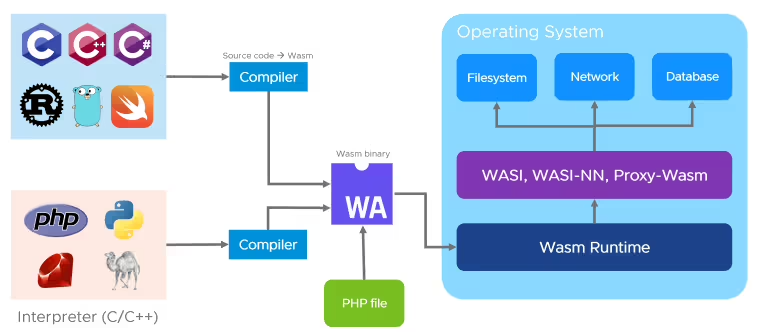
\includegraphics[width=1\textwidth]{images/wasm_compiler.png}
  \caption{Source code gets compiled to the Wasm architecture. The Wasm runtime executes the Wasm bytecode. \cite{docker_without_containers}}
  \label{fig:wasm_compiler_frontend}
\end{figure}

\begin{figure}[H]
  \centering
  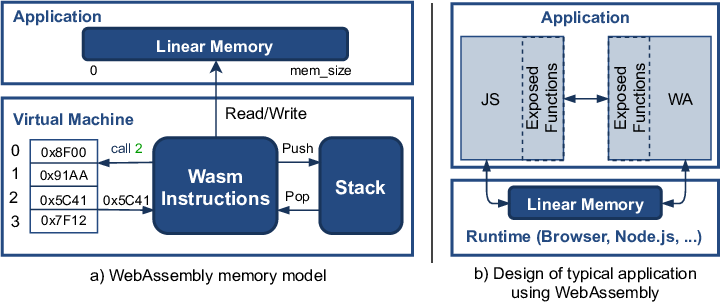
\includegraphics[width=1\textwidth]{images/WebAssembly-high-level-architecture.png}
  \caption{Wasm internals \cite{wasm_vulnerabilities}}
  \label{fig:wasm_high_level}
\end{figure}

\section{\acrshort{WASI}}

When writing code that compiles to Wasm, there is a need for system interfaces. These are required to do useful stuff, such as getting access to files. In the browser, WebAssembly applications can use Javascript as a system interface. However, outside the browser, there is no such predefined system interface. To solve this problem the \acrfull{WASI} was created. \acrshort{WASI} is a set of portable APIs, similar to APIs you would find in an operating system.

\subsection{The Component Model}
\label{section:thecomponentmodel}

A \acrshort{Wasm} program is often build up of multiple libraries called Wasm modules. These modules need a way to talk to each other. They do this by importing and exporting functions. Imported functions are definitions of functions implemented by another Wasm module. If a module calls an imported function, it will be executed by the other module. Exported functions are functions implemented in the module that are exposed to other modules. 
This form of communication is hard to use, as only functions with primitive types are allowed. Passing around more complex data structures, such as strings, lists or structs, is not possible. This is because different programming languages may have different data representations for these structures. For example, a String in Rust may be represented in another way than a String in Python.

To solve this issue, the Component Model was introduced. The Component Model allows users to build applications out of reusable components. These components can be written in different programming languages. Conceptually, a component is a wrapper around a \acrshort{Wasm} module and adds an extra interface layer above the module. This interface is defined with the \acrshort{WIT} language. It does not contain logic, but only describes what a component exports and imports. The \acrshort{WIT} language offers a broader range of primitives compared to \acrshort{Wasm} primitives. For example, strings, enums (ref. variant) and structs (ref. record) can be defined in a \acrshort{WIT}. Subsection \ref{section:WIT} provides further elaboration on WIT.

With the \acrshort{WIT}, components can expose a standardized interface to other components. However, the \acrshort{WIT} only contains the definition of that interface. For correct utilization of this interface, the components should conform to the \acrshort{WIT} in a standardized way. The Canonical \acrshort{ABI} was created to account for this. The Canonical \acrshort{ABI} defines the binary representation of the types used in the \acrshort{WIT}. This way, when one module sends data to another module, the other module can identify what data has been sent. The Canonical \acrshort{ABI} also defines the format of the \acrshort{WIT} types, such as how strings are represented in bytes. Each acrshort{WASI} component should thus make sure that the data it sends conforms to the ABI. This would be tedious for someone creating a component. To solve this issue, tools are created to generate bindings. These tools are tailored to specific programming languages, generating types and interfaces that seamlessly integrate with the idiomatic patterns of each language. The resulting bindings facilitate the conversion of language-specific data types to adhere to the Canonical ABI standard when transmitting to other components. Conversely, upon receiving data from external sources, the bindings ensure the conversion back to the corresponding language-specific types.

\subsubsection{Component kinds}
\label{section:component_kinds}
The Component Model allows components to depend on other components. A distinction of what kinds of components exist is made. Two kinds of components exist.

\paragraph{Command Component}
A Command component is conceptually similar to a regular program on a machine. It has an entry point function labeled \texttt{\_start}, which acts like a \texttt{main} function. This function is called when the component is ran. A command component can depend on reactor components, but not vice versa.

\paragraph{Reactor Component}
A Reactor component is conceptually similar to a library in other programming languages. Contrary to Command components, it does not contain a \texttt{\_start} function. Instead, it exports functions and interfaces, which can be called by other Reactor or Command components.


\subsection{\acrfull{WIT}}
\label{section:WIT}

As briefly described in subsection \ref{section:thecomponentmodel}, the \acrfull{WIT} contains a definition of an interface a \acrshort{WASI} component exposes. It defines this interface in worlds and interfaces. The \acrshort{WIT} does not contain an implementation, but only defines the contract between components. This subsection will briefly discuss the basics of the \acrshort{WIT} language.

\paragraph{World}
A world can be seen as the entrypoint of a component: it contains all the imports and exports of a component. Interfaces and functions can be imported and exported. Exports are what the component provides for other components. Imports are interfaces or functions the component requires. Imports may come from the component itself or from others. Finally, a world can also include another world, essentially being a superset of that world and using all its imports and exports.

A world can also reference interfaces of other packages. For example, the following code snippet imports and exports the interface \texttt{incoming-handler} of package \texttt{wasi:http}:
\begin{verbatim}
world http-proxy {
    export wasi:http/incoming-handler;
    import wasi:http/outgoing-handler;
}
\end{verbatim}

The example file uses the world \texttt{resource-aggregates}. It imports the \texttt{test} interface, which is described in the same file. This means that the interface is included in that specific world. This is necessary, because a wit file can contain multiple worlds, which may not all use the same interfaces. The world will also export the \texttt{test} interface. This means that other components can interact with this component by using the types and functions in the \texttt{test} interface.

\paragraph{Interface}
An interface is a group of types and functions. An interface can represent a certain feature in a library or semantically group a set of elements together. Interfaces declared in other packages can also be used in an interface. This can be done by using the \texttt{use} syntax:
\begin{verbatim}
interface test {
  use wasi:http/incoming-handler@0.2.0{handle};
}
\end{verbatim}

In this example:
\begin{itemize}
\item \textbf{\texttt{test}}: An interface we define.
\item \textbf{\texttt{wasi:http}}: The package that contains the interface \texttt{incoming-handler}.
\item \textbf{\texttt{incoming-handler}}: An interface in the \texttt{wasi-http} package. Note that this interface must be imported in each world that contains the \texttt{test} interface.
\item \textbf{\texttt{0.2.0}}: The version of the \texttt{wasi-http} package.
\item \textbf{\texttt{handle}}: A function we want to use, contained in the \texttt{incoming-handler} interface.
\end{itemize}

The example file contains the \texttt{test} interface.

\paragraph{Types}
The WIT language offers a handful of types, which can be defined in two parts:
\begin{itemize}
\item Built-in primitives: For example, \texttt{u32}, \texttt{string}, \texttt{list<T>} or \texttt{option<T>}.
\item User-defined types: These types are built on top of the primitive types provided by WIT. WIT provides different data structures to define custom types:
\begin{itemize}
\item \texttt{enum}: An enum in WIT is a classic enum type, equivalent to C-style enums:
\begin{verbatim}
enum color {
  blue
  green
  yellow
}
\end{verbatim}

\item \texttt{variant}: Variants are similar to enums, but can have data added to each case. It can be thought of as a combination of an enum and a union.
\begin{verbatim}
variant file-tree-item {
  file(file),
  folder(string, list<file>),
  symlink(string)
}
\end{verbatim}

\item \texttt{record}: Records are equivalent to C structs. They contain a set of fields, each having a name and a type. A record only contains data, and cannot have functions.
\begin{verbatim}
record file {
  id: string,
  name: string,
  contents: data,
  headers: list<header>
}
\end{verbatim}

\item \texttt{flags}: The \texttt{flags} type is an efficient representation of multiple boolean values. It will use a bitset to represent the values.

\begin{verbatim}
flags file-permissions {
  read,
  write,
  execute
}
\end{verbatim}

\end{itemize}
\end{itemize}


\paragraph{Functions}
A WIT function is equivalent to functions in regular languages. It can contain parameters and a return value.
In this example, the function \texttt{lookup} takes parameters \texttt{store} of type \texttt{kv-store} and \texttt{key} of type \texttt{string}. It will return an optional \texttt{string}.

\begin{verbatim}
lookup: func(store: kv-store, key: string) -> option<string>;
\end{verbatim}

\paragraph{Resources}
A resource is a handle to an object in another component. The resource contains functions that are callable upon the associated object. Calling a function on the resource is equivalent to calling a function on an existential type, a concept seen in other languages like Rust or Haskell \cite{haskell_existential}. An existential type implements the resource requirements, but the type is not known. This makes resources different from other WIT types: instead of passing data around, they allow components to \textit{access} objects from other components.

In the example below, the resource \texttt{file-handle} contains 5 functions, which can be put into two categories:
\begin{itemize}

\item static functions: functions \texttt{constructor} and \texttt{default} are static functions. These do not have a reference to an instance of the resource, but are equivalent to regular functions, except that they are namespaced under \texttt{file-handle}. The \texttt{constructor} function will create a new instance of the type and is just syntactic sugar for a regular static function:
\begin{verbatim}
equiv-to-constructor: static func(file: file) -> file-handle
\end{verbatim}

\item instance functions: \texttt{read}, \texttt{seek} and \texttt{write} are instance functions and are called on an already-existing instance which conforms to the resource. An instance function can be desugared into
\begin{verbatim}
seek: func(self: borrow<file-handle>, offset: s32) -> u32;
\end{verbatim}

\end{itemize}

 
\begin{verbatim}
resource file-handle {
    constructor(file: file);
    read(n: u32) -> result<list<u8>, handle-error>;
    seek(offset: s32) -> u32;
    write(data: list<u8>) -> result<_, handle-error>;
    
    default: static func() -> file-handle;
}
\end{verbatim}


\subsection{Milestones}
\acrshort{WASI} is still in development and far from complete. In order to track the development of WASI, its creation has been split up in multiple milestones.

\paragraph{Preview 1}
\acrshort{WASI} Preview 1 was launched in 2019 and marked the first significant milestone in improving WebAssembly interaction outside the browser. Preview 1 contains methods to interact with the file system and command line, resembling a subset of the \acrfull{POSIX} interface. The API is offered to \acrshort{Wasm} modules via the witx \acrfull{IDL}.

\paragraph{Preview 2}
\acrshort{WASI} Preview 2 diverges from the classic \acrshort{POSIX} interface and introduced the Component Model. The Component Model fixes design issues and brings multiple improvements compared to a \acrshort{POSIX} interface, such as having to rely less on file descriptors and being able to use high-level value types instead of unstructured data \cite{path_to_components}. Existing APIs have been rebased to work with the \acrshort{WIT} language and the component model. Preview 2 is currently the latest preview.

\paragraph{Preview 3}
\acrshort{WASI} Preview 3 will bring smaller but important updates to the \acrshort{WIT} language. It is expected to introduce the \texttt{future} and \texttt{stream} keywords in the \acrshort{WIT} language, which adds the ability to express asynchronous functions in the interface. This will bring improvements to existing components which currently rely on polling.

\paragraph{WASI 1.0}
The main goal of \acrshort{WASI} 1.0 is to have a stable runtime which offers stable WIT interfaces to interact with various parts of the system, such as the filesystem. The most important proposals, such as \texttt{wasi-io} and \texttt{wasi-http}, must reach stage 5 of the standardization process \footnote{https://github.com/WebAssembly/WASI/blob/main/Proposals.md} before WASI 1.0 can be launched. 